\documentclass{article}
\usepackage{FinalYearProjectReport}

% packages for references
\usepackage{cite}
\usepackage{url}


% uncomment this line to double line spacing for proof reading
% \linespread{2}

% packages and settings for graphics
\usepackage[pdftex]{graphicx}
\graphicspath{{./}}
\DeclareGraphicsExtensions{.png}
\usepackage[final]{pdfpages}


\title{YOUR TITLE GOES HERE}
\name{YOUR NAME GOES HERE}
\address{Department of Electrical and Computer Engineering\\
University of Auckland, Auckland, New Zealand}


\hyphenation{and-roid}


\begin{document}

\begin{titlepage}
{%\centering
{
\Large
Department of Electrical \& Computer Engineering \\
Final Year Research Project 2013, Final Report}
}
\newline
\newline
\newline

% notes on latex tables use "&" as colum sperator
\begin{table*}[h]
\begin{tabular}{ll}
Project Title: & <<COMPLETE>> \\
Project Number: & <<COMPLETE>> \\
Supervisor Name: & <<COMPLETE>> \\
Second Examiner Name: & <<COMPLETE>> \\
Your Name: & <<COMPLETE>> \\
Your UID: & <<COMPLETE>> \\
Partner Name: & <<COMPLETE>>  \\
Date submitted: & <<COMPLETE>> \\

\end{tabular}
\end{table*}
\begin{table}


\end{table}
\pagebreak
{\Large Declaration of Originality}
\newline
\newline
\newline
This report is my own unaided work and was not copied from 
nor written in collaboration with any other person.

Name: <<COMPLETE>> 


\end{titlepage}




\maketitle



\begin{abstract}
This is where the abstract goes its a little bit different than a normal section.

% use more than one line space for a new paragraph

If you don't use sublime text with the \LaTeX tools plugin you are a \#pleb
\end{abstract}



\section{Introduction}

Put some text here if you want to get a good grade


\section{Section Title}
You might want to cite some references in your report i hear the markers like that.
Use \\cite\{[citation name]\} to cite things like this: \cite{coachseye} \cite{kinovea}.
You will find it auto creates a bibliography at the bottom with all the cites you use in the correct order.

% \newpage only takes you to the top of the next column, to go to a totally new piece of paper you might need to \newpage's
\clearpage
% if you want to get a totally new pice of paper

\section{Section Two}
Having multiple sections increase the chance of you getting an A.
You might want to include picutes as well.
If you want to quote something use backticks then what you want then a normal double quote.
e.g. ``Text'' because using normal double quotes looks silly "ASD"

Images look like this
Include images like this:
\begin{figure}[!h]
\centerline{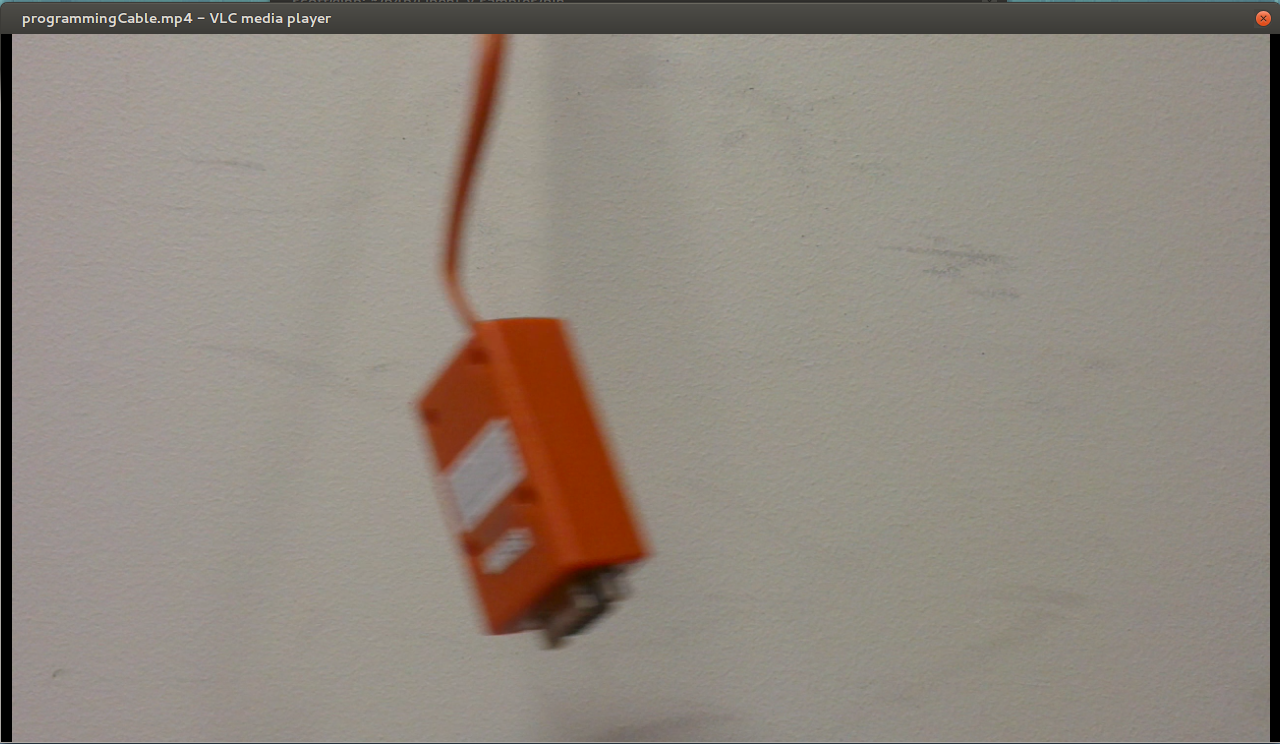
\includegraphics[height=1.8in]{ss1}}
\caption{Desktop application frame from video stream}
\label{fig:rawFrame}
\end{figure}


You can put images at different places on the page by changing the thing after \textbackslash begin\{figure\}[!h].
``!h'' is for Here, and will place it in the page right there.
``!t'' is for Top, and will place it at the top of the column.
``!b'' is for Bottom, and will place it at the bottom of the column.
changing \{figure\} to \{figure*\} will let the figure span the entire page.
You can refrence pages using \textbackslash ref\{label\} \ref{fig:rawFrame}.





\section{Conclusions}
You might want some of these.




\bibliographystyle{IEEEtran}
\bibliography{final_report}


\end{document}